\documentclass{beamer}
\usepackage{graphicx}
\usepackage{amsmath}

\title{Seleção Ótima de Cobertura Sentinel-2 para APAs: Pré-seleção Gulosa de Grupos e Otimização MILP com Fator de Qualidade}
\author{Luryan Delevati Dorneles}
\date{\today}

\begin{document}

\frame{\titlepage}

\begin{frame}
    \frametitle{Objetivos}
    \begin{itemize}
        \item Selecionar imagens Sentinel-2 para cobrir APAs em Alagoas, priorizando dados óticos (no período de 04/12/2024 a 05/04/2025).
        \item Aplicar abordagem híbrida: heurística construtiva gulosa para pré-seleção e modelo MILP para escolha final.
        \item Penalizar o uso potencial de dados SAR (Sentinel-1) como fallback, representando custo adicional.
        \item Balancear cobertura útil e qualidade (cobertura de nuvens, resolução, órbita).
    \end{itemize}
\end{frame}

\begin{frame}
    \frametitle{Trabalhos Relacionados}
    \begin{columns}
        \column{0.5\textwidth}
        \textbf{Otimização em Sensoriamento Remoto}
        \begin{itemize}
            \item \textbf{Kuck et al. (2024)}: Algoritmo genético para priorização de imagens SAR na Amazônia
            \item \textbf{Zhao et al. (2019)}: Programação de satélites com restrições operacionais
        \end{itemize}
        
        \column{0.5\textwidth}
        \textbf{Seleção de Imagens para Mosaicagem}
        \begin{itemize}
            \item \textbf{Li et al. (2018)}: Heurística construtiva para minimizar costuras visíveis
            \item \textbf{Wang et al. (2021)}: Algoritmo guloso para otimizar cobertura espacial
        \end{itemize}
    \end{columns}
    
    \vspace{0.5cm}
    \centering
    \textbf{Gap}: Ausência de abordagens híbridas (heurísticas + métodos exatos)
\end{frame}

\begin{frame}
    \frametitle{Caracterização dos Satélites}
    \begin{columns}
        \column{0.5\textwidth}
        \begin{figure}
            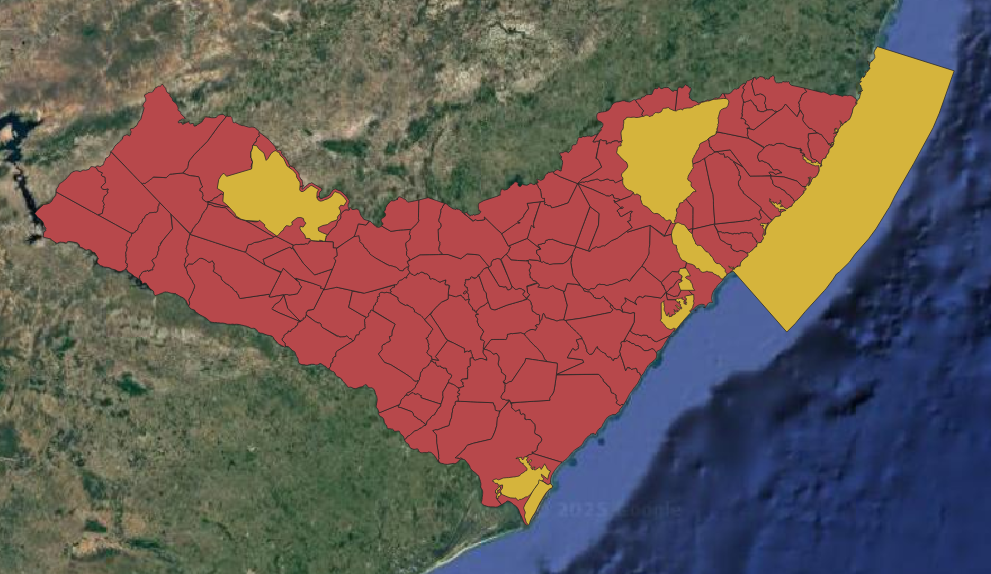
\includegraphics[width=\linewidth]{images/areas.png}
            \caption{Áreas de Proteção Ambiental em Alagoas}
        \end{figure}
        
        \column{0.5\textwidth}
        \begin{itemize}
            \item \textbf{Sentinel-1 (SAR)}:
            \begin{itemize}
                \item Banda C (4-8 GHz)
                \item Penetra nuvens
                \item 5x20m resolução
            \end{itemize}
            \item \textbf{Sentinel-2 (Óptico)}:
            \begin{itemize}
                \item 13 bandas espectrais
                \item 10m resolução
                \item Órbitas regulares (R001-R143)
            \end{itemize}
        \end{itemize}
    \end{columns}
\end{frame}

\begin{frame}
    \frametitle{Metodologia: Abordagem Híbrida}
    \begin{columns}
        \column{0.5\textwidth}
        \textbf{Fase 1: Heurística Gulosa}
        \begin{itemize}
            \item Classificação de imagens (centrais/complementos)
            \item Identificação de combinações para mosaicos
            \item Avaliação multi-critério
        \end{itemize}
        
        \column{0.5\textwidth}
        \textbf{Fase 2: MILP}
        \begin{itemize}
            \item Seleção final de imagens/grupos
            \item Consideração de restrições globais
            \item Otimização da cobertura total
        \end{itemize}
    \end{columns}
    
    \vspace{0.3cm}
    \centering
    \fbox{\begin{minipage}{0.8\textwidth}
    \centering
    Heurística reduz espaço de busca $\rightarrow$ MILP para otimalidade
    \end{minipage}}
\end{frame}

% SLIDE 1: RESTRIÇÕES DE CAPACIDADE
\begin{frame}
    \frametitle{Restrições do Modelo MILP: Capacidade}
    \textbf{Restrições de Capacidade:}
    {\small \begin{align}
        \sum_{g \in G} y_g &\leq N_{\max} \\
        \sum_{t \in T} g_{j,t} &\leq 1, \quad \forall j \in J
    \end{align}}
    \begin{itemize}\setlength{\itemsep}{0pt}\small
        \item $N_{\max}$: Máximo de grupos permitidos
        \item $g_{j,t}$: Ativação do satélite $j$ no tempo $t$
        \item $J$: Conjunto de satélites disponíveis
        \item $T$: Janelas temporais consideradas
    \end{itemize}
\end{frame}

% SLIDE 2: RESTRIÇÕES DE CONSISTÊNCIA
\begin{frame}
    \frametitle{Restrições do Modelo MILP: Consistência}
    
    \textbf{Restrições de Consistência:}
    {\small \begin{align}
        y_g &\leq \sum_{i \in g} x_{i,t}, \quad \forall g \in G, t \in T(g) \\
        \sum_{i \in I_{\text{SAR}}} x_{i,t} &\leq M \cdot g_{j,t}, \quad \forall j \in J, t \in T
    \end{align}}
    \begin{itemize}\setlength{\itemsep}{0pt}\small
        \item $y_g$: Seleção do grupo $g$
        \item $x_{i,t}$: Seleção da imagem $i$ no tempo $t$
        \item $g_{j,t}$: Ativação do satélite $j$ no tempo $t$
        \item $T(g)$: Período válido para o grupo $g$
        \item $I_{\text{SAR}}$: Conjunto de imagens SAR
        \item $M$: Constante grande (Big-M)
    \end{itemize}
\end{frame}

% SLIDE 3: RESTRIÇÕES DE DOMÍNIO
\begin{frame}
    \frametitle{Restrições do Modelo MILP: Domínio}
    
    \textbf{Restrições de Domínio:}
    {\small \begin{align}
        y_g, x_{i,t}, g_{j,t} \in \{0,1\}
    \end{align}}
    \begin{itemize}\setlength{\itemsep}{0pt}\small
        \item $y_g$: Grupo $g$ é selecionado (1) ou não (0)
        \item $x_{i,t}$: Imagem $i$ é adquirida no tempo $t$ (1) ou não (0)
        \item $g_{j,t}$: Satélite $j$ é ativado no tempo $t$ (1) ou não (0)
    \end{itemize}
\end{frame}
\begin{frame}
    \frametitle{Cobertura Efetiva e Classificação de Imagens}
    \begin{align}
    C_i &= C_g \times P_x 
    \end{align}
    
    \begin{itemize}
        \item $C_i$: Cobertura efetiva da imagem
        \item $C_g$: Cobertura geográfica (área ou \%) 
        \item $P_x$: Porcentagem de pixels válidos
    \end{itemize}

    \vspace{0.3cm}
    \textbf{Classificação:}
    \begin{itemize}
        \item \textbf{Imagens Centrais}: $C_i > \theta_{central}$ (30\%)
        \item \textbf{Imagens Complemento}: $C_i$ entre $\theta_{complement}$ e $\theta_{central}$ (7-30\%)
    \end{itemize}
\end{frame}

\begin{frame}
    \frametitle{Função de Avaliação Multi-Critério}
    \begin{align}
    E &= C_n \times Q \\
    C_n &= C_a + C_e + B_o \\
    Q &= (1 - C_c) \times P_x
    \end{align}

    \begin{itemize}
        \item $E$: Efetividade total da combinação
        \item $C_n$: Cobertura normalizada
        \item $Q$: Fator de qualidade
        \item $C_a$: Cobertura atual
        \item $C_e$: Cobertura extra (contrib. da imagem)
        \item $B_o$: Bônus de órbita
        \item $C_c$: Cobertura de nuvens
    \end{itemize}
    
    \textbf{Bônus de órbita:}
    $B_o = 0.1$ se mesma órbita, $0$ caso contrário
\end{frame}

\begin{frame}
    \frametitle{Modelo MILP - Função Objetivo (Implementada)} % Ajustado

    \begin{align}
    \textrm{maximizar} \sum_{g \in G} (E_g \times Q_g \times y_g) - \alpha \sum_{g \in G} y_g - \beta \sum_{g \in G} y_g \label{eq:obj_func_impl}
    % Nota: O termo beta é aplicado a todos os y_g selecionados, pois 'contains_sar' é True para todos os grupos no JSON.
    % A variável teórica x_i,t foi substituída por y_g na implementação.
    \end{align}

    \begin{itemize}\setlength{\itemsep}{0pt}\small
        \item $y_g$: Seleção do grupo de mosaico $g$.
        \item $E_g$: Efetividade (cobertura estimada total) do grupo $g$.
        \item $Q_g$: Qualidade média do grupo $g$.
        \item $\alpha$: Peso para penalizar o \textbf{número de grupos} selecionados.
        \item $\beta$: Peso para penalizar a seleção de \textbf{qualquer grupo} (representando o custo/desincentivo de potencialmente precisar do SAR como fallback). % Ajustado
        % Itens removidos: I_SAR, x_i,t
    \end{itemize}
    \textit{\footnotesize Foco: Maximizar cobertura de qualidade, penalizando o número de grupos ($\alpha$) e a seleção de cada grupo ($\beta$) como peso para o custo de usar SAR.} % Ajustado
\end{frame}

\begin{frame}
    \frametitle{Resultados Preliminares}
    \begin{columns}
        \column{0.5\textwidth}
        \textbf{Estatísticas de Processamento}
        \begin{itemize}
            \item Total de imagens: 328
            \item Imagens aceitas: 94 (29\%)
            \begin{itemize}
                \item Centrais: 50
                \item Complementos: 44
            \end{itemize}
            \item Grupos de mosaicos: 52
        \end{itemize}
        
        \column{0.5\textwidth}
        \textbf{Imagens Rejeitadas: 234 (71\%)}
        \begin{itemize}
            \item Cobertura geográfica insuficiente: 164
            \item Cobertura efetiva insuficiente: 53
            \item Excesso de nuvens: 17
        \end{itemize}
    \end{columns}
\end{frame}

\begin{frame}
    \frametitle{Visualização dos Mosaicos}
    \begin{columns}
        \column{0.48\textwidth}
        \begin{figure}
            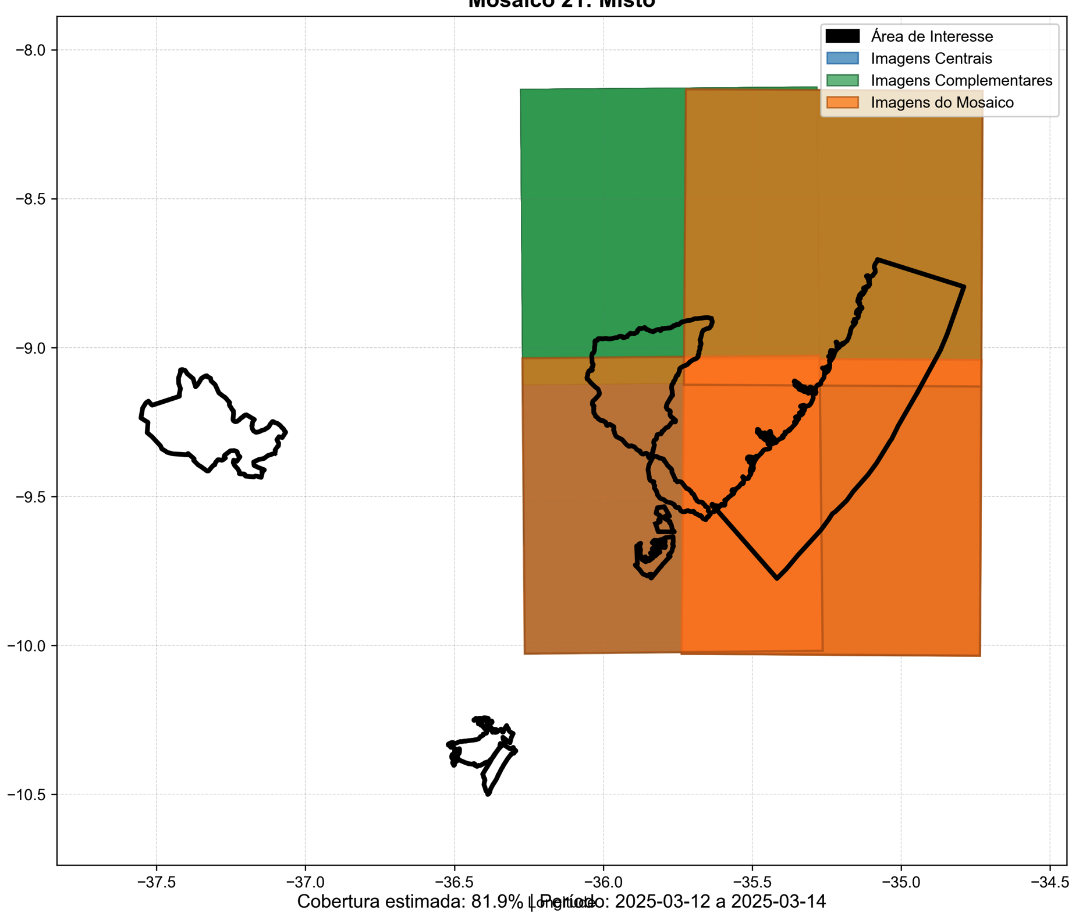
\includegraphics[width=\linewidth,height=3.8cm,keepaspectratio]{images/mosaico.png}
            \caption{\footnotesize Exemplo de mosaico}
        \end{figure}
        
        \column{0.48\textwidth}
        \begin{figure}
            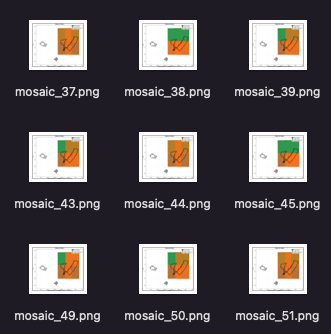
\includegraphics[width=\linewidth,height=3.8cm,keepaspectratio]{images/mosaicos.png}
            \caption{\footnotesize Distribuição de grupos}
        \end{figure}
    \end{columns}
\end{frame}

\begin{frame}
    \frametitle{Detalhamento dos Resultados}
    \begin{columns}
        \column{0.55\textwidth}
        \textbf{Estrutura do JSON:}
        \begin{itemize}\setlength{\itemsep}{0pt}
            \item \textbf{Arquivo}
            \item \textbf{Cobertura Geográfica}
            \item \textbf{Porcentagem de Pixels Válidos} 
            \item \textbf{Cobertura Efetiva} 
            \item \textbf{Cobertura de Nuvens} 
            \item \textbf{Data}
            \item \textbf{Órbita}
        \end{itemize}
        
        \column{0.45\textwidth}
        \begin{figure}
            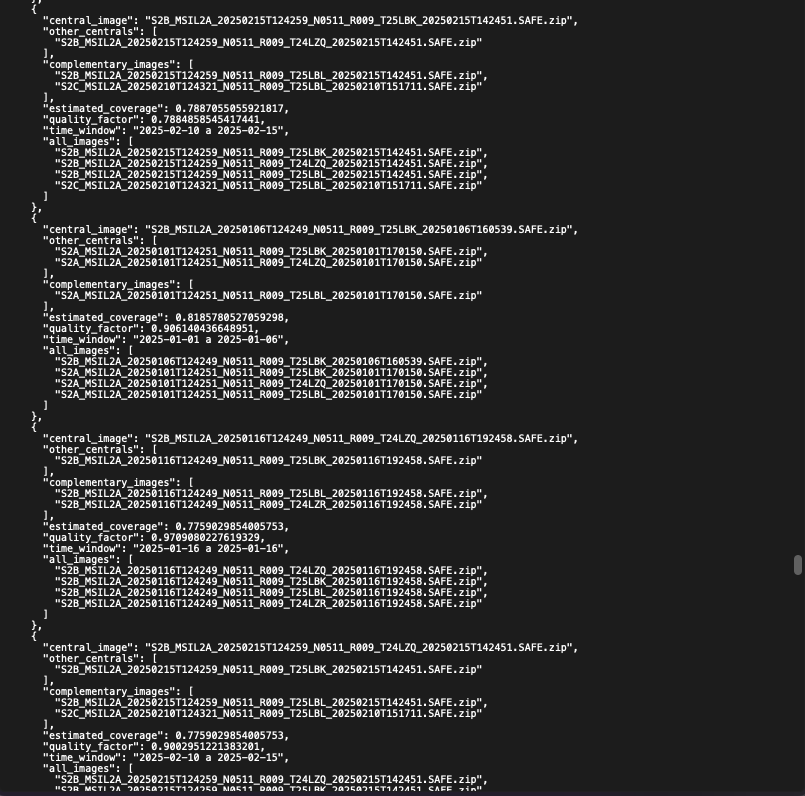
\includegraphics[width=\linewidth,height=4cm,keepaspectratio]{images/json.png}
            \caption{\footnotesize Estrutura de dados do JSON}
        \end{figure}
    \end{columns}
\end{frame}

% Slide com cobertura-rgb.png e cobertura-mask.png lado a lado
\begin{frame}
    \frametitle{Cobertura e Máscara de Nuvens}
    \begin{columns}
        \column{0.5\textwidth}
        \begin{figure}
            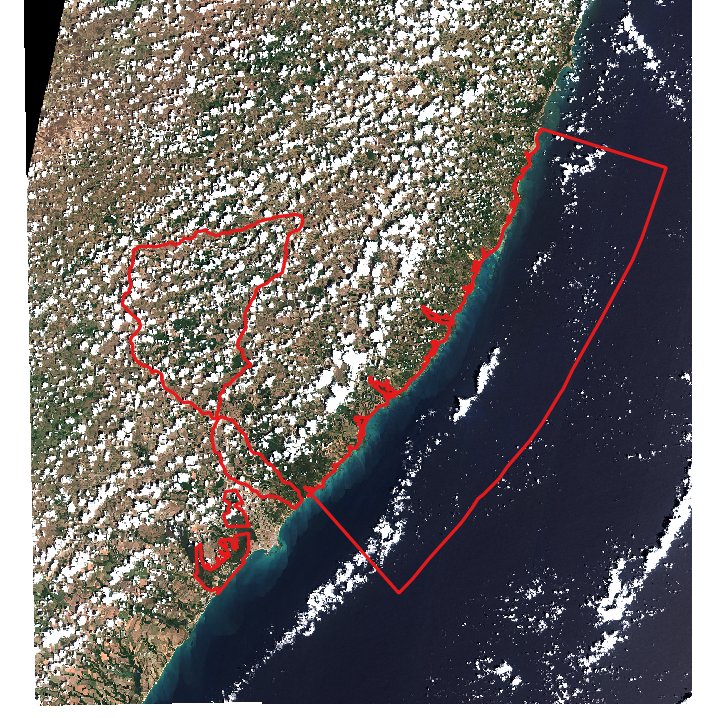
\includegraphics[width=\linewidth,height=6cm,keepaspectratio]{images/cobertura-rgb.png}
            \caption{\footnotesize Imagem RGB de cobertura}
        \end{figure}
        
        \column{0.5\textwidth}
        \begin{figure}
            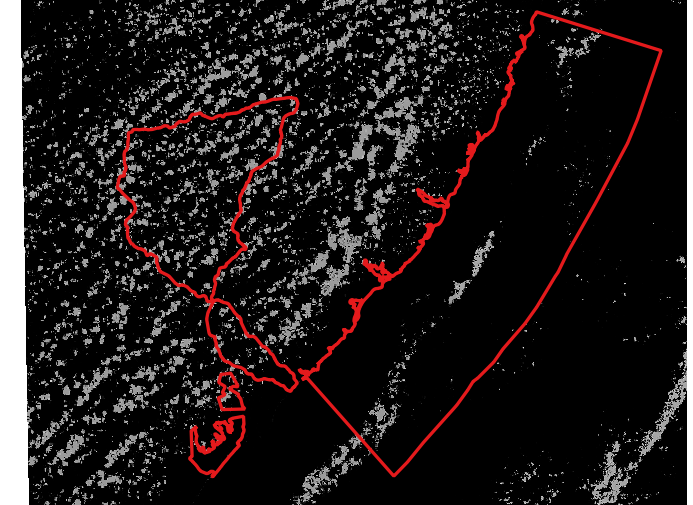
\includegraphics[width=\linewidth,height=6cm,keepaspectratio]{images/cobertura-mask.png}
            \caption{\footnotesize Máscara de nuvens}
        \end{figure}
    \end{columns}
    
    \centering
    \small Comparação entre imagem real e detecção de nuvens para cálculo de cobertura efetiva
\end{frame}

% Slide com zoom1.png (imagem grande única)
\begin{frame}
    \frametitle{Detalhe da Cobertura - Região 1}
    \begin{center}
        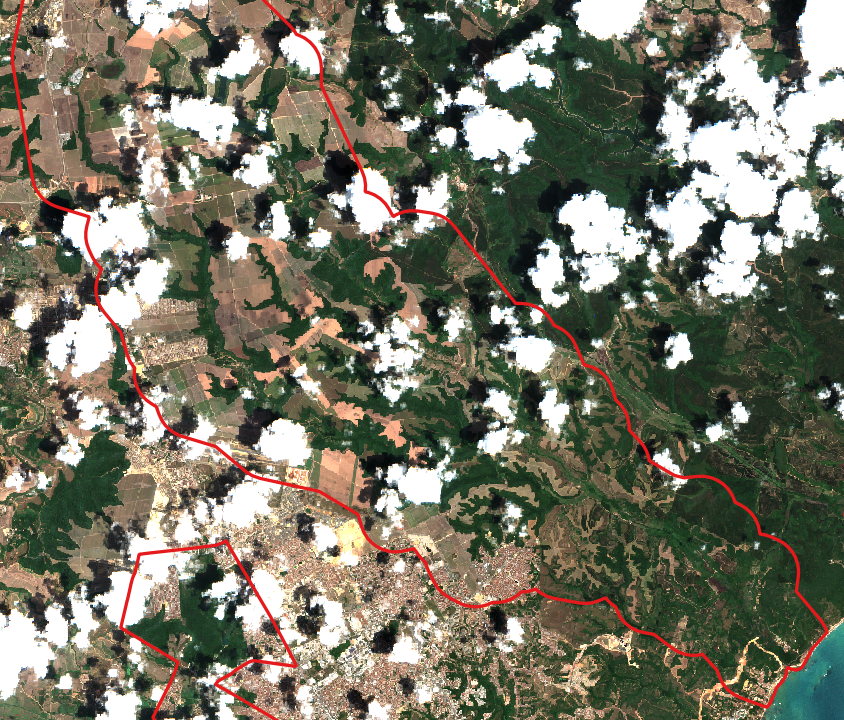
\includegraphics[width=0.9\linewidth,height=7.5cm,keepaspectratio]{images/zoom1.png}
    \end{center}
    
    \centering
\end{frame}

% Slide com zoom2.png (imagem grande única)
\begin{frame}
    \frametitle{Detalhe da Cobertura - Região 2}
    \begin{center}
        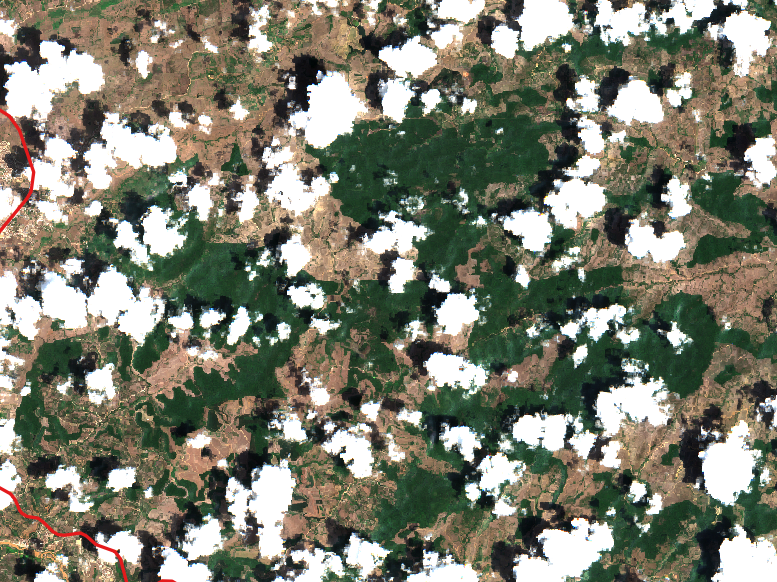
\includegraphics[width=0.9\linewidth,height=7.5cm,keepaspectratio]{images/zoom2.png}
    \end{center}
    
    \centering
\end{frame}

\begin{frame}
    \frametitle{Desafio: Alta Cobertura de Nuvens}
    \begin{center}
        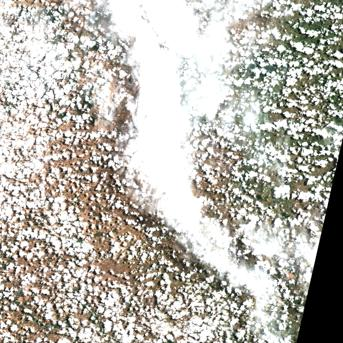
\includegraphics[width=0.85\linewidth,height=7cm,keepaspectratio]{images/muitanuvem.jpg}
    \end{center}
    
    \centering
    \small Exemplo de imagem com alta cobertura de nuvens: descartada pela heurística (baixa cobertura efetiva)
\end{frame}

\begin{frame}
    \frametitle{Conclusão}
    \begin{itemize}
        \item A abordagem híbrida (heurística + MILP) equilibra eficiência computacional e solução de alta qualidade.
        \item Testada com 328 imagens reais (dez/2024 - abr/2025), cobrindo APAs sob diferentes níveis de nuvem.
        \item Heurística filtra e agrupa candidatos (foco em Sentinel-2); MILP refina solução com penalização para SAR.
        \item Solução final maximiza cobertura válida, respeitando restrições e custos.
    \end{itemize}
    
    \vspace{0.3cm}
    \centering
    \textbf{Abordagem híbrida $\rightarrow$ Maximiza cobertura útil com recursos limitados}
\end{frame}

\begin{frame}
    \frametitle{Referências}
    \begin{thebibliography}{9}
        \bibitem{kuck2024} Kuck et al. (2024). Otimização da aquisição de dados SAR para monitoramento de áreas com alto risco de desmatamento no bioma Amazônia com uso de algoritmos genéticos.
        
        \bibitem{zhao2019} Zhao et al. (2019). Programação de satélites de observação da Terra com restrições.
        
        \bibitem{li2018} Li et al. (2018). Heurística construtiva para minimizar costuras visíveis entre imagens adjacentes.
        
        \bibitem{wang2021} Wang et al. (2021). Algoritmo guloso para otimizar a cobertura espacial.
    \end{thebibliography}
\end{frame}

\end{document}